%!TEX root = ../hbrs-poster.tex
\block{Results}
{
	Questions distribution by Relevance and Difficulty for each model
    \begin{tikzfigure}
        \vspace*{-1cm}
        \hspace*{-3cm}
        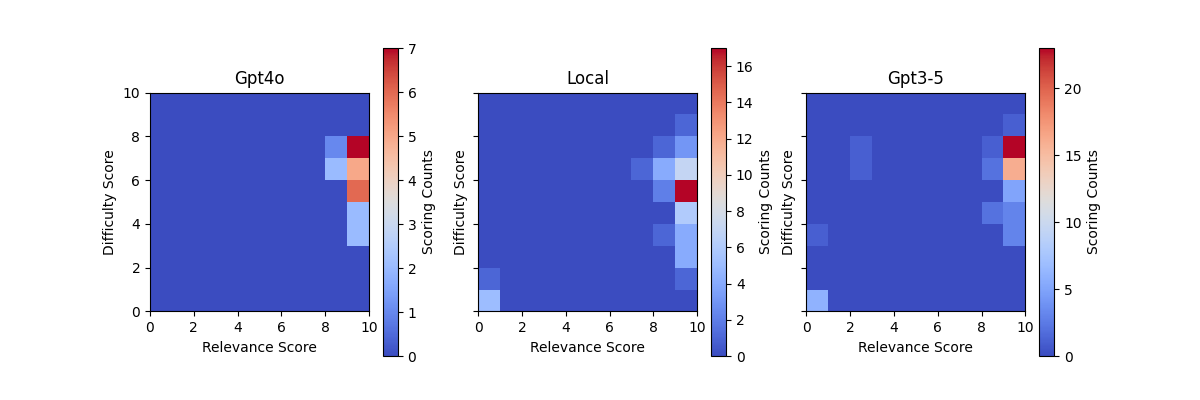
\includegraphics[height=10cm]{figures/eval_plot.png}
    \end{tikzfigure}
    \vspace*{-2.5cm}
}


\block{Contact}
{
	\vspace*{1cm}
	\begin{minipage}{0.75\linewidth}
		\vspace*{-2.5cm}
		Saknini Mohammad, Darius Arbabha, Shinas Shaji\newline
		Hochschule Bonn-Rhein-Sieg\newline
		Email: firstname.lastname@smail.inf.h-brs.de\newline
	\end{minipage}
	\begin{minipage}{0.24\linewidth}
		\centering
		\vspace{-1.5cm}
		\begin{tikzfigure}
			
\includegraphics[scale=0.125]{figures/qrcode.eps}
		\end{tikzfigure}
		Github Repository
	\end{minipage}
	\vspace*{-3cm}
	
}
\block{Acknowledgement}
{
	
	Thanks to Prof. Dr. Jörn Hees and Tim Metzler for the materials and the insightful lecture \textbf{Natural Language Processing}.\newline
	We want to also thank Fraunhofer INT for allowing us to use an OpenAI API key for this project.
}